\documentclass[a4paper,11pt]{article}

\usepackage{exptech}
\usepackage{textcomp}
\usepackage{graphicx}
\usepackage{array}
\usepackage[babel=true]{csquotes}
\usepackage{url}
\usepackage{hyperref}
\hypersetup{
  bookmarks=true, % show bookmarks bar?
  pdftitle={Avalon - Rapport de pré-étude}, % title
  pdfnewwindow=true, % links in new window
  colorlinks=true, % false: boxed links; true: colored links
  linkcolor=black, % color of internal links (change box color with linkbordercolor)
  citecolor=cyan, % color of links to bibliography
  filecolor=cyan, % color of file links
  urlcolor=cyan % color of external links
}

\title{
  \textbf{Avalon}\\
  Rapport de pré-étude
}
\markright{Avalon - Rapport de pré-étude}
\author{
\begin{minipage}{0.4\textwidth}
	\begin{flushleft} \large
		\emph{Auteurs :}\\
		Alexandre \textsc{Audinot}\\
		Julien \textsc{Bouvet}\\
		Cyrille \textsc{Delabre}\\
		Thierry \textsc{Gaugry}\\
		Nicolas \textsc{Hurman}\\
		Léo \textsc{Jacoboni}\\
		Alexandre \textsc{Leonardi}\\
	\end{flushleft}
\end{minipage}
\begin{minipage}{0.4\textwidth}
	\begin{flushright} \large
		\emph{Encadrants :} \\
		Valérie \textsc{Gouranton}\\
		Ronan \textsc{Gaugne}\\
		Bruno \textsc{Arnaldi}\\
		Willy \textsc{Allègre}\\
		Jean-Paul  \textsc{Departe}\\
	\end{flushright}
\end{minipage}
}

\date{23 Octobre 2014}

\begin{document}
\maketitle
\thispagestyle{empty}
\begin{abstract}
\textbf{Avalon :} Environnement de Réalité Virtuelle pour l'apprentissage à l'utilisation d'appartements tremplins. Réalisation en 3D d'un appartement domotisé interactif utilisé dans le cadre de la rééducation des personnes handicapées.
Le projet est proposé par le centre mutualiste de rééducation et de réadaptation fonctionnelles de Kerpape (plus particulièrement Willy Allègre et Jean-Paul Departe et sera réalisé à l'aide de Unity3D et MiddleVR.
\end{abstract}

\vfill

\begin{figure}
   \begin{minipage}{0.3\linewidth}
      
\includegraphics[width=\textwidth]{1-PreEtude/img/logo_insa.jpeg}
   \end{minipage} \hfill
   \begin{minipage}{0.3\linewidth}
      
\includegraphics[width=\textwidth]{1-PreEtude/img/logo_kerpape.png}
   \end{minipage}
   \begin{minipage}{0.3\linewidth}
      
\includegraphics[width=\textwidth]{1-PreEtude/img/logo_irisa.jpg}
   \end{minipage}
\end{figure}

\pagebreak

\tableofcontents
\pagebreak

\section{Contexte}

\subsection{Qu'est-ce que la réalité virtuelle ?}La notion de réalité virtuelle, contrairement à ce que l'on pourrait penser, n'est pas récente et date du début des années 80 quand Jaron Lanier, un informaticien américain pionnier du domaine, l'a popularisée. Cette notion n'a pourtant pas, à l'origine, l'exact sens qu'on lui prête habituellement aujourd'hui : une réalité virtuelle sous-entendrait qu'il s'agit d'une copie exacte de la réalité, ce qui n'est jamais le cas, faute de moyens techniques, et n'est pas toujours recherché. Le terme venant  de l'anglais, \emph{virtual} peut se traduire par \emph{virtuelle} mais aussi par \emph{quasi} ou \emph{pratiquement}, or cette notion de \emph{quasi-réalité} correspondrait mieux à ce qu'est effectivement la réalité virtuelle. \\

En effet, de manière plus formelle, on peut définir la réalité virtuelle comme suit :

\begin{quote}\og \emph{La réalité virtuelle est un domaine scientifique et technique exploitant l'informatique et les interfaces comportementales en vue de simuler dans un monde virtuel le comportement d'entités 3D, qui sont en interaction en temps réel entre elles et avec un ou des utilisateurs en immersion pseudo-naturelles par l'intermédiaire de canaux sensori-moteurs.} \fg{}\end{quote}\cite{traiteRV1}

%Il faudra penser à citer la source : Le traité de la RV
Cela signifie que pour que l'on puisse parler de réalité virtuelle il faut que plusieurs conditions soient réunies :
\\
\begin{itemize}\renewcommand{\labelitemi}{$\bullet$}
\item \textbf{La présence d'interfaces comportementales et sensorielles. }
Les interfaces comportementales désignent les interfaces entre l'utilisateur et le monde virtuel. Il existe dans un premier temps des interfaces motrices, qui permettent de reconnaître les différentes actions que l'utilisateur peut entreprendre (mouvements, voix, etc). Ainsi le système informatique gérant le monde virtuel peut alors les prendre en compte. Les interfaces sensorielles font ensuite la liaison opposée et informent l'utilisateur de l'état du monde virtuel et des modifications éventuelles des actions entreprises précédemment (images, sons, etc). La réciprocité du besoin d'une interface motrice et sensorielle, qui sont nécessaires pour l'immersion du sujet et permettent de gérer l'interaction avec le monde virtuel, est illustrée par la \textsc{figure 1}.
\item \textbf{L'immersion du sujet.}
L'immersion caractérise le fait que les interfaces entre l'utilisateur et le monde virtuel doivent se faire oublier, et ce, en ressemblant le plus possible aux méthodes d'interaction que nous avons avec le monde réel. Elle ne peut pas être parfaite, car il y a toujours du matériel à utiliser qui n'est pas nécessaire pour interagir avec le monde réel (lunettes 3D, WiiMote, etc) mais doit être la plus totale possible.\\

\end{itemize}
\begin{figure}
  \caption{Interactions entre monde réel et virtuel \cite{traiteRV1}}
  %\centering
  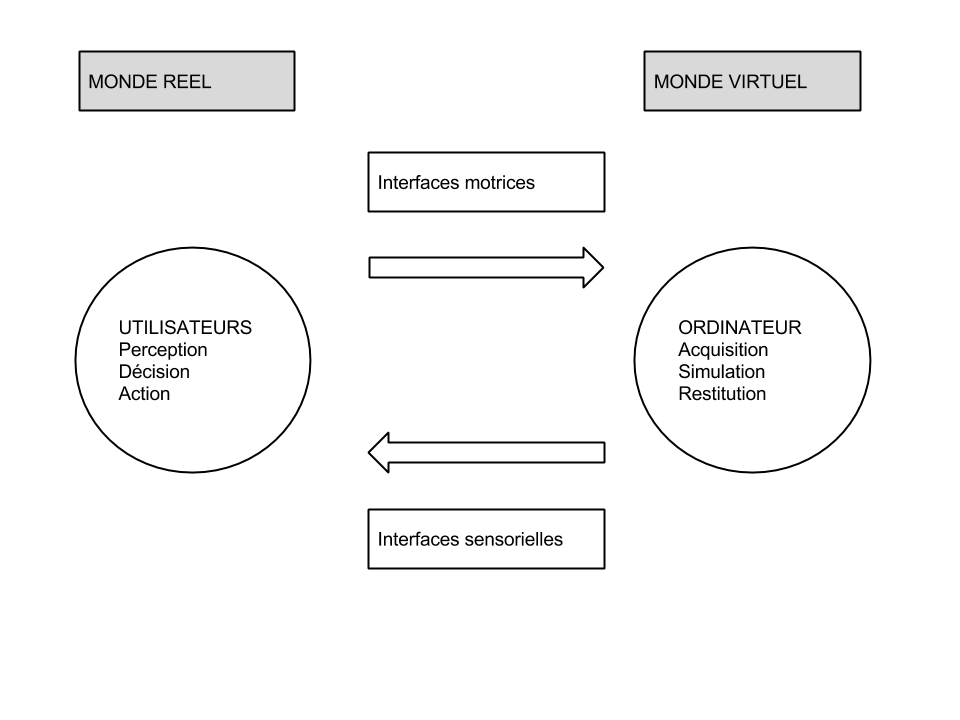
\includegraphics[scale=0.4,bb=0 0 720 720]{1-PreEtude/img/graphe_interfaces.png}
\end{figure}

La notion de réalité virtuelle implique donc également celles d'immersion et d'interaction, elles sont en fait constitutives de ce qu'est la réalité virtuelle. L'utilisateur doit pouvoir faire des actions motrices sur son environnement, il doit pouvoir agir dessus que ce soit par les mouvements, la parole, les gestes... Il n'y a pas de règles définies tant qu'il s'agit d'une activité motrice.
Une activité sensorielle, par ailleurs, signifie que l'utilisateur percevra un impact de ses actions sur le monde virtuel. Encore une fois il n'y a pas de liste de réponses sensorielles acceptables, ce peut être un son ou encore une modification de l'affichage.


\subsection{La Réalité Virtuelle et l'aide à la personne}

\subsubsection{L'aide à la personne}

Notre projet va traiter d'une application bien particulière de la réalité virtuelle (RV) : la santé. La RV est déjà utilisée dans le cadre de la santé et des soins. Les psychologues s'en servent par exemple pour traiter les cas de phobie, car une application de réalité virtuelle leur permet de plonger leurs patients dans la situation qui est l'objet de leur peur facilement, mais aussi de la garder sous contrôle et de la reproduire rapidement et à peu de frais. Le même avantage s'applique au traitement de l'autisme chez les enfants, car la RV permet de simuler des situations qui s'avéreraient dangereuses et qu'ils ne savent pas gérer, comme traverser une route seuls.\cite{traiteRV4}\\

Notre projet a été proposé par le centre de rééducation et de réadaptation fonctionnelle de Kerpape, et se focalisera donc sur le domaine d'expertise du centre, à savoir l'aide aux personnes handicapées. Le principe de l'aide à la personne est d'assister des personnes âgées ou handicapées dans les gestes de tous les jours, pour leur permettre de conserver leur autonomie.

\subsubsection{Le centre de Kerpape}

Nous avons eu l'occasion de visiter le centre de Kerpape au cours de notre projet. Kerpape accueille 400 patients chaque jour, et a pour objectif de leur permettre d'acquérir l'autonomie nécessaire à une réinsertion sociale et professionnelle. \\
Du fait de la grande diversité des handicaps que présentent les patients du centre, la modification du matériel existant est un pan important du travail de Willy Allègre et Jean-Paul Departe, les ingénieurs commanditaires de notre projet, et cela rend la RV particulièrement intéressante, un logiciel étant plus facilement reconfigurable que du matériel.\cite{kerpape}\\


C'est le second projet de RV auquel participe le centre de Kerpape. Le premier était le projet AGATHE, débuté en 2009, dont le but est d'aider les personnes atteintes de troubles cognitifs (par exemple dus à la maladie d'Alzheimer, à des AVC, ...) à être autonomes dans la vie de tous les jours. Le projet consiste en la réalisation d'un \og voisinage virtuel \fg{} dans lequel le patient peut se déplacer, et où se trouvent plusieurs points d'intérêts avec lesquels il peut interagir, tel qu'un bureau de poste, un supermarché, etc. Le patient a donc accès à différentes actions en accord avec le lieu dans lequel il se trouve, et le thérapeute peut évaluer ses performances en fonction de plusieurs critères comme le temps passé par le patient dans une zone donnée.\cite{agathe}

\subsubsection{Le projet Avalon}

Le projet qui nous a été confié, le projet Avalon, est le premier projet de collaboration entre Kerpape et l'INSA. Il a aussi pour but d'aider les personnes handicapées à recouvrer leur autonomie, mais il se focalise sur un aspect différent de la vie de tous les jours : l'utilisation de la domotique dans l'habitat des patients. Durant leur phase de rééducation au centre de Kerpape, les patients sont amenés à vivre quelques temps dans un appartement \enquote{tremplin} appartenant au centre. Ces appartements sont lourdement équipés en domotique pour que des personnes handicapées puissent y être autonomes, les différentes portes, fenêtres et volets sont contrôlables à distance par différents interrupteurs, un plan de travail dans la cuisine est réglable en hauteur, un mobile accroché à des rails au plafond aide les déplacements, etc.
Les appartements tremplins servent à présenter aux patients les différents équipement disponibles pour leur propre appartement une fois qu'ils quitteront le centre, mais aussi à les entraîner à l'usage de ces équipements, qui peut s'avérer complexe, particulièrement pour les personnes souffrant de handicaps mentaux. \\

Le centre de Kerpape a donc initié le projet Avalon pour permettre aux patients de se préparer à l'utilisation des appartements même si ceux-ci sont occupés, et pour que les thérapeutes encadrant les patients puissent profiter de différents modes d'utilisation leur permettant de se focaliser sur les interactions les plus problématiques, comme détaillé dans le cahier des charges.

\pagebreak

\section{Cahier des charges}
\subsection{Partie fonctionnelle}
  
Nous avons eu l’occasion d’échanger avec les membres de Kerpape, ce qui nous a permis de définir le cahier des charges de l’application.\newline
En effet, l'utilisation des appartements tremplins qui permet la mise en situation des patients dans un environnement réel, rencontre des difficultés avec les patients ayant des troubles cognitifs. La domotique trés présente dans l'appartement rencontre donc des difficultés de compréhension et d’utilisation de la part des patients, d'où l'idée d'un environement virtuel d'apprentissage en amont.

\subsubsection{Modes de fonctionnement}

Le programme doit comporter trois modes d’utilisation dont deux assistent en partie l’utilisateur pour son apprentissage. Le troisième permet une interaction avec l'environnement de manière plus autonome.
\newline 

\textbf{Apprentissage symbolique}
\newline 

Ce mode doit permettre de tout apprendre depuis le début et de comprendre le fonctionnement global des différentes situations auxquelles l'utilisateur peut être confronté. Il comporte des vues statiques, “zoomées”, avec la mise en évidence d’action à réaliser, ainsi que des indications visuelles symboliques.
\newline 

\textbf{Assisté}
\newline 

Dans un environnement réaliste, le logiciel donne des indications légères pour permettre de retrouver les actions à faire. Ces indications sont activables par les ergothérapeutes. \newline 
Par exemple :\newline 
- la surbrillance des objets à actionner,\newline 
- lors de l'activation d'une action on accède à une vue fixe avec les états courants des équipements afin de faciliter la compréhension action/objet pour l'utilisateur.
\newline 

\textbf{Autonome}
\newline 

L’utilisateur ne reçoit plus d’information ou d’indication pour effectuer son parcours, il est dans le décor le plus réaliste possible, pour valider son autonomie. Il doit alors actionner les différents objets et se rendre compte par lui même (déplacement) des actions qu'il a éffectué.

\subsubsection{Points de vue : endocentré, exocentré}

Deux points de vue sont configurables. Une vue à la troisième personne (exocentrée), et une vue à la première personne (endocentrée).

\subsubsection{Déplacements, mise en situation et interactions}

L'utilisateur peut se déplacer librement dans l'appartement en mode autonome ; en parallèle il peut choisir de se mettre en situation sur les différents scénarios proposé afin d'interragir avec les différents objets prévus pour le scénario. 

Centrées autour d’un bloc d’interrupteurs, les interactions comprennent notamment de pouvoir ouvrir/fermer les portes (porte du hall avec fermeture automatique / porte de l’appartement avec fermeture volontaire), d'allumer/éteindre les lumières (commande variateur / commande ON/OFF) et de monter/descendre les volets.

\subsubsection{Scénarios}
Trois scénarios autour de l'appel sur le téléphone sont à prévoir avec des actions différentes à entreprendre décrites dans l'étude fonctionnelle. 
\newline 

\textbf{Appel téléphonique: }\textit{Appel téléphonique (d’un proche ou d’une personne qui se serait trompée de numéro). }\newline 
%- L'utilisateur doit pouvoir décrocher le téléphone pour entrer en communication puis raccrocher quand la communication est terminée.
%\newline 

\textbf{Interphone infirmier: } \textit{Appel venant du portier audio/vidéo sur le téléphone (d’un infirmier qui souhaiterait entrer). }\newline 
%L'utilisateur doit pouvoir décrocher le téléphone, communiquer avec l'infirmier, raccrocher le téléphone et ouvrir la porte.
%\newline 

\textbf{Interphone inconnu: } \textit{Appel venant du portier audio/vidéo sur le téléphone (d’un inconnu). }\newline 
%L'utilisateur doit pouvoir décrocher le téléphone pour entrer en communication, allumer la TV pour voir la vidéo puis éteindre la TV et raccrocher le téléphone à la fin de la conversation.



 

\pagebreak


\section{Etude fonctionnelle}

La solution logicielle que nous allons implémenter doit intégrer plusieurs scénarios de fonctionnement. Ceux-ci permettront de tester les aptitudes du patient en rééducation dans un contexte banal. Ces scénarios sont axés sur l'interaction entre le patient et le monde extérieur, via le "Domophone". 

\subsection{Scénario 1: Appel téléphonique entrant}

Le premier scénario à implémenter est assez basique. Il s'agit du cas où le résident reçoit un appel téléphonique. Il doit alors décrocher puis raccrocher le téléphone au terme de la conversation.

D'un point de vue logiciel, il s'agira de déclencher la sonnerie du téléphone pour avertir l'utilisateur. Une icône de téléphone peut être affichée en bas de l'écran, dans un coin. Ensuite, l'utilisateur devra se déplacer ver la zone du téléphone. Suivant le mode d'utilisation, le rendu sera différent : En mode symbolique, le logiciel basculera sur une vue du téléphone donnera les instructions pour décrocher puis pour raccrocher. En mode assisté, le téléphone sera en surbrillance et si l'utilisateur met trop de temps pour agir sur le téléphone, certains boutons peuvent se mettre en surbrillance ou clignoter.

\subsection{Scénario 2: Visite de l'infirmier}

Ce scénario correspond à la visite d'une personne connue par le résident. Lorsque que le visiteur arrive, il utilise l'interphone pour demander l'ouverture du portail. Le patient en rééducation doit décrocher le domophone, activer l'ouverture du portail grâce aux interrupteurs et raccrocher. Ce cas correspond bien à la visite d'un infirmier ou d'une quelconque personne que le résident peut reconnaître par la voix. 

Pour cette implémentation la différence avec le scénario 1 portera sur l'ouverture du portail. En effet, après avoir raccroché, l'utilisateur devra se rendre au niveau des interrupteurs et déclencher l'ouverture du portail. En mode symbolique, le basculement entre les vues sera automatique. Le mode assisté mettra en évidence l'ensemble des interrupteurs, puis en cas d'hésitation, le bon interrupteur sera mis en valeur.

\subsection{Scénario 3: Visite d'un inconnu}

Le scénario le plus complet correspond au passage d'un visiteur inconnu. En effet, le résident devra dans cette situation décrocher le téléphone, puis activer l'affichage vidéo de l'interphone sur l'écran de télévision de l'appartement. Ensuite, il devra vérifier qu'il peut laisser entrer le visiteur et le cas échéant, lui ouvrir le portail grâce aux interrupteurs, puis raccrocher. S'il ne désire pas lui ouvrir, il lui faudra juste raccrocher.
Ce scénario convient à plusieurs situations courantes : visite d'un réparateur, d'un livreur, d'un témoin de Jéhovah ...

Pour réaliser la partie "`visio TV"' de ce scénario l'utilisateur va devoir : activer la vision via le domophone, allumer la télévision et éteindre la télévision. Là encore, les 3 modes de fonctionnement vont modifier le comportement du logiciel et orienter plus ou moins l'utilisateur vers la télévision. En mode symbolique, l'utilisateur sera guidé pas à pas pour : 
\begin{itemize}
	\item activer la visio depuis le domophone
	\item allumer la télévision
	\item éteindre la télévision
\end{itemize}
La suite du scénario reprend le fonctionnement final du scénario 2, qui lui-même reprend la fin du scénario 1.

\subsection{Diagramme des cas d'utilisation}
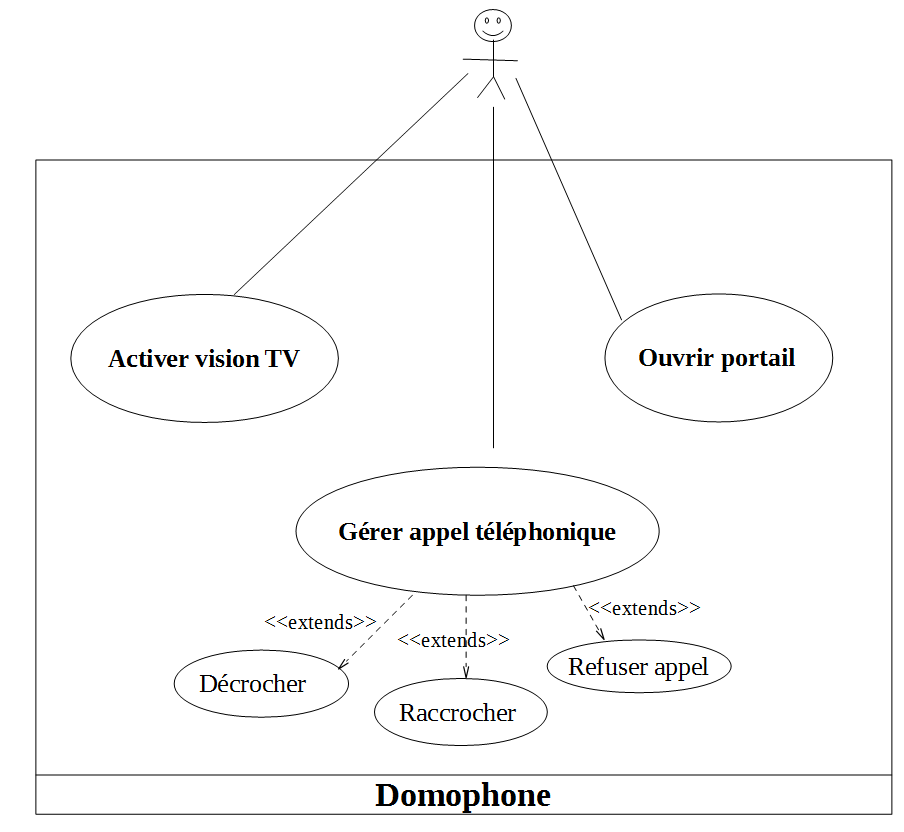
\includegraphics[scale=0.5]{1-PreEtude/img/use_case_diag}

\pagebreak
\input{1-PreEtude/etude-technique.tex}
\pagebreak
\section{Sp\'ecifications}

\subsection{Données}
	D'autres travaux on déjà été réalisés : http://infositu.loria.fr/ >> domotique + RV + aide personne
	Pour ce projet, nous avons à notre disposition une modélisation 3D de l'appartement tremplin. Cette modélisation, fournie par Kerpape, est au format .max.
	- format de Unity (fbx)
	Applications de la réalité virtuelle en sciences de la vie :
	Le traitement de troubles de stress post-traumatique (TSPT)
	Le traitement de phobies
	Le traitement d'addictions
	Le contrôle de la douleur des grands brûlés
	Les études comportementales et de perception
	L'éducation à la santé publique
	La formation à l'anatomie, aux pathologies et à la chirurgie pour les étudiants et médecins
	La cyberanatomie
	...et bien d'autres encore.

%	http://fr.wikipedia.org/wiki/Th%C3%A9rapie_par_r%C3%A9alit%C3%A9_virtuelle
%	http://www.fhpmco.fr/2014/08/27/des-lunettes-a-realite-augmentee-pour-aider-les-malvoyants
%	http://www.pourlascience.fr/ewb_pages/a/article-realite-virtuelle-pour-therapies-reelles-21783.php
\subsection{Logiciels}
	Au cours de ce projet, nous allons devoir travailler entre différents environnements logiciels; ceux-ci entrent dans deux grandes catégories : les modeleur 3D et les autres trucs.
	Voici les solutions logicielles que nous allons utiliser pour la réalisation de notre projet :
	
	\subsubsection{3DSmax}
		3DSmax, le célèbre modeleur 3D d’Autodesk n’est plus à présenter; aujourd’hui considéré comme la référence en matière de modélsation 3D, et ce depuis plus de 10 ans, il est grandement utilisé dans l’industrie vidéoludique et filmographique
	
	\subsubsection{Blender} 
		Blender, son alternative libre. Soutenue par la fondation blender, qui a par ailleurs réalisé quelques films d’animations tels que Big Buck Bunny ou Sintel, ses fonctionnalitées ne sont plus à prouver.
	
	\subsubsection{Unity} 
		Unity est un environnement et un moteur de rendu 3D ; initialement pensé pour les jeux vidéos, il permet de créer ou modifier des environnements en 3D et correspond parfaitement à nos besoins pour la modification du modèle d’appartement tremplin.
		De plus, contrairement à d’autres moteurs 3D, Unity propose une version gratuite, qui regroupe la majorité des fonctionnalités de la version payante à l'exception de la compilation 64b et ???.
		Il permet de réaliser toutes les actions classiques d'un logiciel de ce type, comme construire des objets, les animer, interagir avec, etc. Toutes ces actions sont effectuées de manière native depuis l'interface en écrivant des scripts C# ou Javascript via l'API fournie.
		Le développement y est grandement facilité, car celle-ci inclus de nombreuses fonctionnalités.
		Il n'y a donc pas besoin de sortir du logiciel pour développer.
		Unity est actuellement utilisé dans la salle Immersia de l’Irisa.      

	\subsubsection{VRPN}
		VRPN (Virtual-Reality Peripheral Network) est un système de gestion de périphériques pour la réalité virtuelle. Cette bibliothèque offre une interface entre le matériel et l'application. Elle offre des classes génériques pour chaque type de périphériques; par exemple, tout les trackers sont gérés de la même façon.
		Le projet fut initié en 1998 par Russell M. Taylor II de l'université de Caroline du Nord et est aujourd'hui maintenu par une vingtaine de contributeurs.
	
	\subsubsection{MiddleVR}
		MiddleVR est un plugin compatible avec Unity qui s'appuit sur  VRPN. Développé par I’m in VR (PARIS, France) permettant de gérer les interactions entre l’utilisateur et son environnement, et spécialement conçu pour les environnements en réalité virtuelle. 
		L'objectif de MiddleVR est de pouvoir programmer l'application en s'abstrayant des spécificités matérielles pour qu'elle soit déployable partout.
		Il propose une couche d’abstraction entre les périphériques et Unity. Ces périphériques comprennent ceux d’entrée (de capture), tels que les classiques claviers et souris mais aussi les bras à retour de force ou des MS Kinect, ainsi que ceux de sortie (de restitution), comme les écrans, les vidéoprojecteurs 3D mais aussi le son ou le retour de force des bras. 
		MiddleVR gère nativement la stéréoscopie active ou passive,
		- Interaction devices like 3D trackers (see full list on the right),
		- Clustering: Scenelock, swaplock both sofware \& hardware,
		- 3D interactions: Navigation, manipulation, menus and custom graphical user interfaces
		MiddleVR = s'abstraire des interfaces homme-machine - 

	\subsubsection{\#Five}
		\#Five est une bibliothèque pour Unity developpée en interne au sein de l’Irisa. \#Five ajoute plusieurs couches, parmi lesquelles : 
		Donner la mécanique qui fait les relations entre les objets pour gérer réactivité
		Infrastructure gérant le travail collaboratif sur environnement virtuel, c'est à dire quand plusieurs personnes intéragissent sur la même scène.
		Scénario de haut niveau, si je veux démonter une culasse, il faut démonter les boulons, pour démonter les boulons : Si je fais le 1 alors ensuite il faut faire le X, mais si je fais le 2 en premier alors il faut faire le Y ensuite
		Objets réactifs (décor, objets, inter relations) + scénario + humains virtuels pouvant collaborer


\subsection{Matériels et environnement technique}

Ce projet consistant en l'utilisation d'un environnement 3D virtuel (appartement de Kerpape aidant à la réhabilitation de personnes lourdement handicapées), où l'utilisateur sera amené à avoir des interactions avec cet environnement, nous allons donc avoir accès à la salle de réalité virtuelle $\mu$RV de l'INSA Rennes et à son matériel. à nous d'utiliser ce dernier à bon escient, pour répondre au mieux à la demande de Kerpape et pour pouvoir proposer un environnement d'apprentissage le plus performant possible notamment au niveau des interactions avec l'utilisateur. 
Ci-dessous vous trouverez la présentation du matériel présent dans la salle $\mu$RV et l'intérêt que pourrait présenter leur utilisation dans le projet.

\subsubsection{Matériel d'immersion}
Nous disposons de différents outils pour immerger l'utilisateur au coeur de l'environnement virtuel : 
\\

\textbf{Lunettes nVidia 3D Vision et Récepteur 3D Vision}
\\

Ces lunettes, sur batterie, permettent de visualiser une stéréoscopie active. Elles sont reconnues par l'ordinateur grâce à une base quiémet des signaux infrarouges.
\\

\textbf{Lunettes 3D Vuzik Wrap 920}
\\

Les lunettes 3D Vuzix Wrap 920 disposent de deux écrans intégrés ainsi que d'un capteur de mouvements.
\\

\textbf{Vidéoprojecteur 3D}
\\

Le vidéoprojecteur permet d'avoir un écran 3D à disposition pour s'immerger dans l'environnement plus facilement avec une qualité graphique bien supérieure à celle d'un écran d'ordinateur classique.
\\


\textbf{Oculus Rift}
\\

Le dispositif se démarque des systèmes comparables expérimentés précédemment par la très courte latence dans le suivi des mouvements de la tête et par l'important champ de vision offert. L'appareil se présente sous la forme d'un masque recouvrant les yeux et attaché au visage par une sangle ferméeà l'arrière du crâne. Un écran plat numérique est placéà quelques centimètres en face des yeux, perpendiculairementà l'axe du regard. Cet écran affiche une image stéréoscopique déformée numériquement pour inverser la distorsion optique créée par deux lentilles situées en face de chaque œil. Divers capteurs permettent de détecter les mouvements de tête de l'utilisateur, ce qui permet d'adapter en temps réel l'image projetée sur l'écran, afin de produire l'illusion d'une immersion dans la scène restituée.
\\

\textbf{Plateforme Immersia}
\\

En forme de « L », la salle Immersia est dotée d'un équipement immersif plongeant l?utilisateur dans un monde visuel et auditif de haute qualité. 
Elle est constituée  :
\begin{itemize}
  \item d'un système visuel utilisant 11 projecteurs : 8 Barco Galaxy NW12 et 3 Barco Galaxy 7+.
  \item d'un écran de verre de 9,60 mètres de long où sont projetées par l?arrière, les images stéréoscopiques.
  \item d'un système de localisation ART permettant à des objets réels d?être localisés à l?intérieur de la plate-forme.
  \item d'un système de rendu sonore fourni par un processeur Yamaha, lié soit à des hauts-parleurs Genelec au format sonore 10.2, soit à des casques Beyer Dynamic avec un format sonore virtuel de 5.1, contrôlé par la position de l?utilisateur.
\end{itemize}

\subsubsection{Matériel d'interaction}
Une fois l'utilisateur intégré dans la modélisation virtuelle de l'appartement, nous avons à notre disposition plusieurs équipements pour le faire interagir avec son environnement :
\\

\textbf{Microsoft Kinect}
\\

La Kinect développée par Microsoft, est le périphérique le plus intéressantà exploiter dans le cadre de la réalité virtuelle. Elle permet en effet de détecter la présence de 6 personnes et de suivre les mouvements de deux utilisateurs actifs grâceà ses lentilles placées sur un socle motorisé. Sa portée est comprise entre 1,2m et 3,5m. L'intérêt principal de la Kinect est que l'utilisateur puisse se déplacer librement dans une pièce sans avoirà manipuler une quelconque manette.
\\

\textbf{WiiMote, Nunchuck et WiiMotionPlusInside}
\\

La Wiimote est la manette fournie avec la console de jeu Wii, développée par Nintendo. Elle est composée de deux parties : la manette principale et le Nunchuk. Bien que moins pratique que la Kinect (l'utilisateur est contraint de manipuler une manette), la Wiimote dispose d'un système de liaison bluetooth d'une portée de 10m permettant une utilisation sans fil. L'avantage de la Wiimote réside dans le nombre et la précision des informations qu'elle est capable de fournir au programme. 
\newline
Elle permet en effet de :
\begin{itemize}
  \item mesurer les accélérations selon 3 axes (axes naturels 3D) grâces aux accéléromètres placés dans la manette principale et le Nunchuk
  \item mesurer l'inclinaison de la manette principale selon les 3 axes naturels
  \item mesurer la distance ainsi que la position entre la Wiimote et la barre infrarouge (référentiel).
\end{itemize}

\textbf{Joystick Extreme 3D Pro Logitech}
\\

Avec ses commandes avancées et sa gouverneà manche rotatif, ce joystickà retour de force stable et précis est prévu pour être connecté à un ordinateur et est utilisé pour des jeux de combat aérien acrobatique. Il est composé d'une gouverneà manche rotatif et de nombreux boutons.
\\

\textbf{Bras à retour de force Novint Falcon}
\\

Le Falcon, de la société Novint, est un périphérique haptique branché en USB. Il permet de ressentir le retour d'effort, et donc la texture et la résistance des objets, leur poids... Une boule est reliée au support par des tiges. C'est elle que l'on déplace et qui transmet à la main de l'utilisateur les efforts des moteurs.
\\

\subsection{Techniques d'interaction}
Au vu de toutes les ressources technologiques dont nous disposons, nous avons décidé de privilégier les techniques d'interaction suivantes :

\subsubsection{Interface Clavier/Souris et écran d'ordinateur}
Une première version utilisable sur un ordinateur avec ses périphériques de base (clavier et souris) permettant d'avoir un environnement d'apprentissage fonctionnel et testable rapidement, et également très portable.

\subsubsection{Compatibilité avec tous les périphériques via MiddleVR}
L'objectif serait de présenter une application fonctionnant avec tous les périphériques à notre disposition et cités précédemment, grâce à une reconnaissance et une configuration automatique des périphériques.
\\

\pagebreak
\section{Planification}
\subsection{Versions intermédiaires}
Lors de la réalisation de ce projet, nous allons produire plusieurs versions intermédiaires pour nous permettre de construire chaque fonctionnalité au fur et à mesure.
\subsection{Organisation du travail}
Pour ce projet, nous avons mis en place un certain nombre d'outils de travail collaboratif :

\begin{itemize}
  \item GitHub : pour nos documents versionnés tel que le code source
  \item Cloud privé : pour les documents confidentiels
  \item Google Drive : pour tout autre document
  \item Wiki : 
\end{itemize}


\subsection{Estimation du planning}
Au cours de l'année, nous sommes chargés de rédiger 6 papiers (rapports, documentation) et de réaliser un certain nombre de versions intermédiaires de notre logiciel.
Voici une estimation du planning pour l'année :

\begin{tabular}{|l|l|}
\hline
  Date &
  Production \\
\hline
  19 Octobre &
  Rapport de spécification fonctionnelle VP \\
\hline
  27 Octobre &
  Rapport de spécification fonctionnelle VF \\
\hline
  9 Décembre &
  Version PC \textnumero1 \\
\hline
  9 Décembre &
  Dossier de planification Initial VP \\
\hline
  16 Décembre &
  Version PC \textnumero2 \\
\hline
  17 Décembre &
  Dossier de planification Initial VF \\
\hline
  6 Février &
  Rapport de conception logicielle VP \\
\hline
  12 Février &
  Rapport de conception logicielle VF \\
\hline
  25 Mars &
  Page HTML VP \\
\hline
  2 Avril &
  Page HTML VF \\
\hline
  16 Mai &
  Documentation en Ligne VP \\
\hline
  21 Mai &
  Rapport Final/Annexes + Bilan Planification \\
\hline
  26 Mai &
  Rapport Final/Annexes + Bilan Planification \\
\hline
  28 Mai &
  Documentation en Ligne VF \\
\hline
\end{tabular}


\pagebreak

\section{Conclusion}
Au cours de cette étude, nous avons eu l'occasion de rencontrer nos interlocuteurs de Kerpape et nous avons pu dresser un premier portrait de la solution technique que nous allons développer.
La prochaine étape va être de mettre en application les solutions évoquées, pour avoir une première version du logiciel permettant de se déplacer librement dans l'appartement. 
Il faut donc importer le modèle dans une scène sous Unity, et y rajouter les lumières ainsi que les éléments manquants (panneau de commandes, téléphone).
Nous redécouperons de manière plus détaillée les tâches à réaliser dans le prochain rapport où nous planifierons l'ensemble de la réalisation technique.

\pagebreak

\bibliography{1-PreEtude/biblio}

\end{document}
